\ExamPart{Trắc nghiệm trả lời ngắn}{2}{Thí sinh trả lời từ câu 1 đến câu 4.}

\NQuestion Cho đồ thị hàm số $y=f\left(x\right)$ như hình vẽ dưới đây.
\begin{center}
    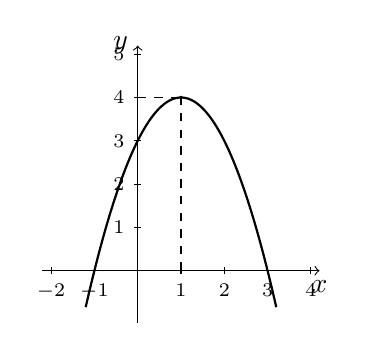
\begin{tikzpicture}[scale=0.55]
    \draw[->] (-2.2,0) -- (4.2,0) node[below] {$x$};
    \draw[->] (0,-1.2) -- (0,5.2) node[left] {$y$};
    \foreach \x in {-2,-1,1,2,3,4}
        \draw (\x,0.08) -- (\x,-0.08) node[below] {\scriptsize $\x$};
    \foreach \y in {1,2,3,4,5}
        \draw (0.08,\y) -- (-0.08,\y) node[left] {\scriptsize $\y$};
    \draw[smooth, samples=200, domain=-1.2:3.2, thick] plot (\x, {-(\x-1)^2+4});
    \fill (1,4) circle (1.2pt);
    \draw[dashed] (1,0) -- (1,4);
    \draw[dashed] (0,4) -- (1,4);
\end{tikzpicture}

\end{center}
Tìm giá trị lớn nhất của hàm số $f\left(x\right)$.
\AnswerLine{$4$}
\SolutionBlock{Từ đồ thị, parabol mở xuống và có đỉnh $I(1;4)$. Do đó giá trị lớn nhất của hàm số là $4$.}

\NQuestion Phương trình $x^4-5x^2+4=0$ có bao nhiêu nghiệm thực phân biệt?
\AnswerLine{$4$}
\SolutionBlock{Đặt $t=x^2\ (t\ge0)$, ta có
\[
t^2-5t+4=0 \Leftrightarrow (t-1)(t-4)=0.
\]
Suy ra $t=1$ hoặc $t=4$. Tương ứng:
\[
x=\pm1,\quad x=\pm2.
\]
Vậy có $4$ nghiệm thực phân biệt.}

\NQuestion Từ các chữ số $0,1,2,3,4,5,6$, lập được bao nhiêu số tự nhiên có $3$ chữ số khác nhau, không bắt đầu bằng $0$ và lớn hơn $300$?
\AnswerLine{$120$}
\SolutionBlock{Xét chữ số hàng trăm. Để số lớn hơn $300$, chữ số hàng trăm phải là $3,4,5$ hoặc $6$, nên có $4$ cách chọn. Với mỗi cách:
\begin{itemize}[leftmargin=1.5em]
\item Chữ số hàng chục có $6$ cách chọn trong các chữ số còn lại;
\item Chữ số hàng đơn vị có $5$ cách chọn tiếp theo.
\end{itemize}
Do đó có $4\cdot6\cdot5=120$ số.}

\NQuestion Một khu vườn hình chữ nhật có chiều dài hơn chiều rộng $5$ m và diện tích bằng $84$ m$^2$. Tính độ dài đường chéo của khu vườn.
\AnswerLine{$\sqrt{193}$}
\SolutionBlock{Gọi chiều rộng là $x$ m, khi đó chiều dài là $x+5$ m. Ta có
\[
x(x+5)=84 \Rightarrow x^2+5x-84=0 \Rightarrow (x+12)(x-7)=0.
\]
Vì $x>0$ nên $x=7$. Khi đó chiều dài là $12$. Đường chéo khu vườn là
\[
\sqrt{7^2+12^2}=\sqrt{49+144}=\sqrt{193}.
\]}
